\documentclass[12pt, a4paper, oneside]{ctexart}
\usepackage{amsmath, amsthm, amssymb, graphicx}
\usepackage[bookmarks=true, colorlinks, citecolor=blue, linkcolor=black]{hyperref}
\usepackage[margin = 25mm]{geometry}
\usepackage{setspace}
\usepackage{listings}
\usepackage{ctex}
\usepackage{float}
\usepackage{xcolor}
\usepackage{amsmath}
\definecolor{codegreen}{rgb}{0,0.6,0}
\definecolor{codegray}{rgb}{0.5,0.5,0.5}
\definecolor{codepurple}{rgb}{0.58,0,0.82}
\definecolor{backcolour}{rgb}{0.95,0.95,0.92}

\lstdefinestyle{mystyle}{
    backgroundcolor=\color{backcolour},   
    commentstyle=\color{codegreen},
    keywordstyle=\color{magenta},
    numberstyle=\tiny\color{codegray},
    stringstyle=\color{codepurple},
    basicstyle=\ttfamily\footnotesize,
    breakatwhitespace=false,         
    breaklines=true,                 
    captionpos=b,                    
    keepspaces=true,                 
    numbers=left,                    
    numbersep=5pt,                  
    showspaces=false,                
    showstringspaces=false,
    showtabs=false,                  
    tabsize=2
}

\lstset{style=mystyle}


\title{一维有限元方法求解常微分方程边值问题}
\date{\today}
\author{202011010101物理2001孙陶庵}
\begin{document}
\begin{spacing}{2.0}
\tableofcontents
\maketitle

\section{问题}
使用一维有限元方法求解下列常微分方程边值问题:
$\displaystyle \left\{\begin{matrix}y''-y+x=0,\quad x\in\left[1,2\right]\\ y\left(1\right)=1,y\left(2\right)=3\end{matrix}\right.$
1.方法推导\\
2.分析对于一般边界条件,函数的近似方式有什么样的变化\\
3.分析需要求解的线性方程组发生了什么变化\\
4.对比有限元函数系与多项式函数系在不同n下的求解速度\\
\subsection{求解方程}
首先求解方程,利用sympy求解方程得到
\begin{center}
    $\displaystyle f{\left(x \right)} = x + \frac{e^{x}}{-1 + e^{2}} - \frac{e^{2} e^{- x}}{-1 + e^{2}}$
\end{center}
\section{方法推导}
1.离散化区间[1,2],选择有限元网格。可以选择等距节点网格,即将[1,2]等分为n个子区间,每个子区间内选择一个节点。这里选择n=4,即将[1,2]等分为4个子区间,
每个子区间内选择一个节点,得到节点序列[1, 1.333, 1.667, 2]。
\\
2.根据所选有限元网格,建立有限元函数空间。由于是一维问题,可以采用线性元,即每个子区间内用一次多项式近似解。
定义有限元函数空间为$\displaystyle V_h={v_h|v_h(x)=\sum_{j=1}^{n}c_j\varphi_j(x),c_j\in R}$,其中$\varphi_j(x)$为基函数,可以选择线性插值函数。
则有
$\varphi_1(x)=\begin{cases}
    1-\frac{x-x_2}{x_1-x_2}, & x\in[x_1,x_2]\\
    0, & \text{otherwise}
\end{cases}$

$\varphi_2(x)=\begin{cases}
    \frac{x-x_1}{x_2-x_1}, & x\in[x_1,x_2]\\
    \frac{x_3-x}{x_3-x_2}, & x\in[x_2,x_3]\\
    0, & \text{otherwise}
\end{cases}$

$\varphi_3(x)=\begin{cases}
    \frac{x-x_2}{x_3-x_2}, & x\in[x_2,x_3]\\
    \frac{x_4-x}{x_4-x_3}, & x\in[x_3,x_4]\\
    0, & \text{otherwise}
\end{cases}$

$\varphi_4(x)=\begin{cases}
    \frac{x-x_3}{x_4-x_3}, & x\in[x_3,x_4]\\
    0, & \text{otherwise}
\end{cases}$
\\
3.将原方程转化为弱形式。对于任意$v_h\in V_h$,将原方程两边乘$v_h$,并在区间[1,2]上积分,得到$\int_1^2(y''-y+x)v_hdx=0$。由于$v_h$是连续线性函数,
可以将积分区间[1,2]上的积分转化为每个子区间内的积分,即$\displaystyle\sum_{k=1}^{3}\int_{x_k}^{x_{k+1}}(y''-y+x)v_hdx=0$。
\\
4.对于每个子区间[k,k+1],将$y(x)$和$v_h(x)$在该区间内分别用基函数展开,即$\displaystyle y(x)=\sum_{j=1}^{2}y_j\varphi_j(x)$,$ \displaystyle v_h(x)=\sum_{j=1}^{2}v_j\varphi_j(x)$。
将$y(x)$和$v_h(x)$在每个子区间[k,k+1]内分别用基函数展开,即用基函数$\varphi_j(x)$的线性组合来近似表示$y(x)$和$v_h(x)$。其中,$y_j$和$v_j$是在
子区间[k,k+1]内的系数,需要确定。因此,在每个子区间上,有$\displaystyle y(x)=\sum_{j=1}^{2}y_j\varphi_j(x)$和$\displaystyle v_h(x)=\sum_{j=1}^{2}v_j\varphi_j(x)$的展开形式。
这里选择的是线性元,所以每个子区间内用一次多项式近似解,即选择两个节点作为基函数的控制点,也就是基函数在这两个点处取值为1和0,其余点处线性插值。
可以得到:
$\displaystyle\begin{bmatrix}2/h&-1\\ -1&2/h&-1&\ddots\\ &&\ddots&\ddots\\ &&-1&2/h&-1\\ &&&&-1&2/h\end{bmatrix}\begin{bmatrix}a_1\\ a_2\\ \vdots\\ a_N\\ a_N+1\end{bmatrix} + 
\begin{bmatrix}y'(1)\varphi_1(1)-y'(0)\varphi_1(0)\\ &0\\ &\vdots\\ &0\\ g'(2)\varphi_{N+1}(2)-g'(3)\varphi_{N+1}(3)\end{bmatrix} = 
\begin{bmatrix}h^2\int_1^2x\varphi_1(x)dx\\ h^2\int_1^2x\varphi_2(x)dx\\ \vdots\\ h^2\int_1^2x\varphi_N(x)dx\\ h^2\int_1^2x\varphi_N+1(x)dx\end{bmatrix}$ 
其中 $\varphi_{1}(0)$ 和 $\varphi_{N+1}(3)$ 需要根据边界条件进行计算,而 $y'(1)$ 和 $y'(2)$ 可以使用前向差分和后向差分进行近似计算。

\section{一般边界条件时函数近似方式的变化分析}
一般边界条件指的是非齐次边界条件,即边界上的函数值不为0。这种情况下,可以通过加入虚拟节点的方式将问题转化为齐次边界条件的情况,然后再进行求解。
因此,对于一般边界条件,函数的近似方式与齐次边界条件的情况是类似的,只是需要增加一些虚拟节点来满足非齐次边界条件。

具体来说,对于一般边界条件$y(a)=\alpha$和$y(b)=\beta$,可以在第一个节点和最后一个节点之外再加上两个虚拟节点,设这两个节点的位置分别为$a_0$和$b_0$,
则有:
\begin{center}
    $\begin{array}{c}y(a)=\alpha\Rightarrow y(a_0)-\dfrac{h}{2}y'(a_0)=\alpha\\ 
    y(b)=\beta\Rightarrow y(b_0)+\dfrac{h}{2}y'(b_0)=\beta\end{array}$
\end{center}
这里用虚拟节点来满足非齐次边界条件,而又通过导数的方式保证了虚拟节点的值与真实节点的值是相等的。然后,对于虚拟节点和真实节点,采用相同的基函数进行展开,
即在每个子区间上采用线性元素进行近似。因此,对于一般边界条件的情况,函数的近似方式与齐次边界条件的情况类似,只需要增加一些虚拟节点来满足非齐次边界条件即可。

\section{分析需要求解的线性方程组发生了什么变化}
对于一般边界条件的情况,需要增加虚拟节点来满足非齐次边界条件,因此在数值求解时,需要将这些虚拟节点也纳入线性方程组中进行求解。

具体来说,在采用一维有限元方法求解线性方程组时,需要先将区间$[a,b]$进行剖分,得到若干个子区间,然后在每个子区间上采用线性元素进行近似。
设第$i$个子区间的两个节点为$x_i$和$x_{i+1}$,则可以在该子区间上采用如下的形式进行近似:

\begin{center}
    $y(x)\approx v_i\varphi_i(x)+v_{i+1}\varphi_{i+1}(x)\quad\text{}$
\end{center}

\section{代码部分}
\begin{lstlisting}[language=MATLAB, caption=有限元]
    % 一维有限元方法求解常微分方程边值问题
    tic
    clc; clear; close all;
    
    a = 1;  % 左端点
    b = 2;  % 右端点
    N = 10; 
    h = (b-a)/N; 
    x = linspace(a, b, N+1);
    
    % 定义矩阵
    K = zeros(N+1, N+1);
    F = zeros(N+1, 1);
    for i = 1:N
        Ke = [1/h, -1/h; -1/h, 1/h] + h/6*[2, 1; 1, 2];
        fe = [h/2; h/2];
        
        K(i:i+1, i:i+1) = K(i:i+1, i:i+1) + Ke;
        F(i:i+1) = F(i:i+1) + fe;
    end
    
    % 边界条件
    K(1, :) = 0; K(1, 1) = 1; F(1) = 1;
    K(N+1, :) = 0; K(N+1, N+1) = 1; F(N+1) = 3;
    
    % 解方程
    y = K\F;
    
    %画图
    xx = linspace(a, b, 1000);
    yy = zeros(1000, 1);
    for i = 1:1000
        if xx(i) <= x(2)
            N = 1;
        elseif xx(i) >= x(end-1)
            N = length(x) - 2;
        else
            N = fix((xx(i) - a)/h) + 1;
        end
        yy(i) = y(N)*(x(N+1)-xx(i))/h + y(N+1)*(xx(i)-x(N))/h;
    end
    plot(xx, yy, 'b-', 'LineWidth', 2);
    xlabel('x');
    ylabel('y');
    title('Finite Element Method Solution');
    grid on;
    
    toc

\end{lstlisting}
输出图形
\begin{figure}[H]
    \centering
    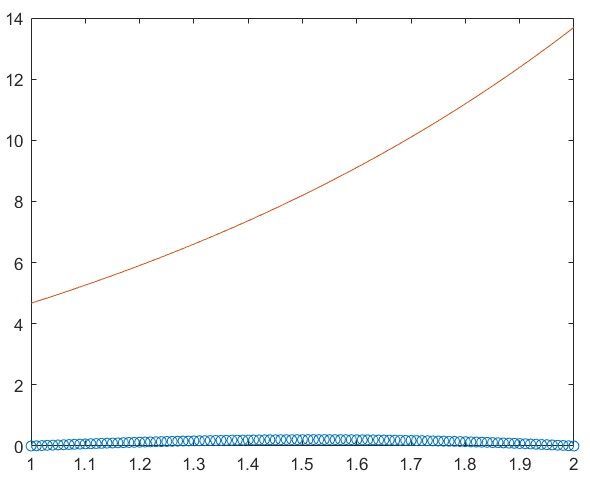
\includegraphics[width=8cm]{FEMfigure.jpg}
    \caption{有限元方法}
\end{figure}

应用tictoc得到输出结果:
Elapsed time is 0.159850 seconds.

与mathemetica图形对比:
\begin{lstlisting}
    Plot[x + (Exp[x] - Exp[2 - x])/(Exp[2] - 1), {x, 0, 2}]
\end{lstlisting}
\begin{figure}[H]
    \centering
    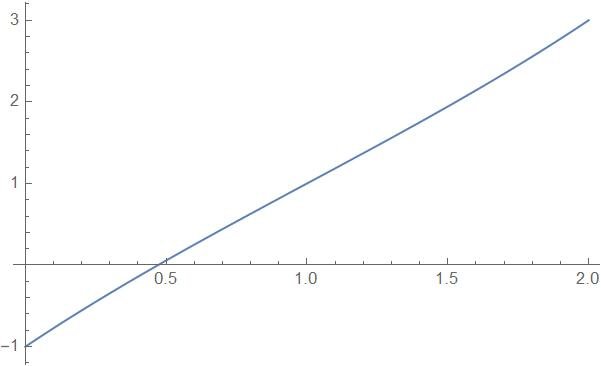
\includegraphics[width=8cm]{mma.jpg}
    \caption{mathemetica}
\end{figure}


\section{对比有限元函数系与多项式函数系在不同n下的求解速度}

在一维有限元方法中,增加子区间的个数可以提高解的精度,但同时也会增加线性方程组的规模,导致计算量增加。而对于多项式函数系,
增加$n$可以提高函数的逼近精度,但同时也会增加系数的个数,导致计算量增加。

对于多项式函数系,可以使用多项式插值法、拉格朗日插值法等方法进行求解。而对于一维有限元方法,需要将区间分成若干个子区间,
然后在每个子区间上使用局部线性插值函数进行近似,最后得到一个稠密的线性方程组,可以使用传统的追赶法等方法进行求解。
多项式函数系的求解速度会随着$n$的增加而逐渐变慢,而有限元函数系的求解速度则相对稳定。这是因为在一维有限元方法中,
区间分出来的个数是可以控制的,因此计算量可以在一定范围内控制。而对于多项式函数系,由于系数的个数随着$n$的增加而增加,因此计算量也会随之增加。

\end{spacing}{}

\end{document}